\documentclass[11pt,a4paper]{article}
\usepackage[utf8]{inputenc}
\usepackage[T1]{fontenc}
% babel-spanish no esta en esta instalacion de TeX Live: se cargan a mano los
% dos ajustes que importan, los rotulos de figura y cuadro en castellano.
\usepackage{lmodern}
\renewcommand{\figurename}{Figura}
\renewcommand{\tablename}{Cuadro}
\renewcommand{\refname}{Referencias}
\renewcommand{\abstractname}{Resumen}
\usepackage[margin=2.6cm]{geometry}
\usepackage{graphicx}
\usepackage{booktabs}
\usepackage[expansion=false]{microtype}
\usepackage{xcolor}
\usepackage[colorlinks=true,linkcolor=azulo,urlcolor=azulo,citecolor=azulo]{hyperref}
\definecolor{azulo}{HTML}{2A78D6}
\usepackage{caption}
\captionsetup{font=small,labelfont=bf}
\setlength{\parskip}{.45em}
\setlength{\parindent}{0pt}

% Generado por informe/numeros.py — no editar a mano.
\newcommand{\AUCMax}{??}
\newcommand{\AUCMediana}{??}
\newcommand{\AUCMin}{??}
\newcommand{\DrugMax}{1\,985}
\newcommand{\DrugMin}{19}
\newcommand{\FechaCorrida}{2026-09-08 16:30}
\newcommand{\NAfiliaciones}{769\,661}
\newcommand{\NAristas}{36\,152\,622}
\newcommand{\NComparadas}{??}
\newcommand{\NCompuestosAntes}{2\,396\,103}
\newcommand{\NCompuestosDespues}{831\,175}
\newcommand{\NDiscrepancias}{??}
\newcommand{\NDruggables}{19\,650}
\newcommand{\NEspecies}{16}
\newcommand{\NEspeciesOpt}{??}
\newcommand{\NExplicadas}{??}
\newcommand{\NIdenticas}{??}
\newcommand{\NInterPro}{14\,083}
\newcommand{\NNegativos}{101\,973}
\newcommand{\NOrthoMCL}{76\,157}
\newcommand{\NPositivos}{248\,545}
\newcommand{\NPromiscuos}{7}
\newcommand{\NProteinas}{399\,353}
\newcommand{\NPruebas}{38}
\newcommand{\NRegistros}{1\,983\,780}
\newcommand{\NSobreAzar}{??}
\newcommand{\PctAristasFiltradas}{1.6}
\newcommand{\VersionPandas}{3.0.5}
\newcommand{\VersionPython}{3.12.11}


\title{\vspace{-1.5cm}Priorización de blancos terapéuticos sobre una red multicapa\\[.3em]
\large Reproducción sobre una base codificada, con la procedencia registrada}
\author{Gonzalo Giordano}
\date{Corrida del \FechaCorrida\ \\[.2em]
\small\url{https://github.com/Gonzalo174/TDR-GW-AI-course}}

\begin{document}
\maketitle

\begin{abstract}
\noindent
Dado el genoma de un organismo, ordenar sus proteínas por cuán prometedoras son
como blanco de un fármaco. La evidencia experimental es escasa y está repartida
de forma muy desigual entre organismos, de modo que la estrategia es propagar lo
que se sabe de unas proteínas a otras sobre una red de tres capas: compuestos,
proteínas y anotaciones funcionales. Este informe reproduce el análisis completo
sobre una versión \emph{codificada} de la base --- toda columna es un entero y los
diccionarios que traducen esos enteros son privados --- y documenta la procedencia
de cada resultado junto con la verificación que lo sostiene. La reproducción
recupera \NIdenticas\ de \NComparadas\ columnas idénticas a un oráculo
independiente, con \NDiscrepancias\ discrepancias.
\end{abstract}

\section{El problema}

Un programa de descubrimiento de fármacos para una enfermedad desatendida
empieza por elegir qué proteína atacar. Esa elección se hace con poca evidencia:
para la mayoría de los organismos de interés se conocen apenas decenas de
proteínas con actividad medida, sobre genomas de miles.

La hipótesis que explota este trabajo es que la evidencia se puede transferir.
Dos proteínas que comparten un dominio funcional tienden a comportarse parecido
frente a un compuesto, y dos compuestos químicamente similares tienden a actuar
sobre las mismas proteínas. Formalizado, eso es una red de tres capas sobre la
que se propaga una señal desde las proteínas con evidencia hacia las que no la
tienen.

La base de este trabajo tiene \NProteinas\ proteínas de \NEspecies\ organismos,
\NPositivos\ enlaces de bioactividad positiva y \NAfiliaciones\ afiliaciones a
\NInterPro\ dominios InterPro y \NOrthoMCL\ grupos de ortología.

\section{Los datos y lo que se les hizo}

La base publicada en el repositorio no es la original: se derivó de ella en tres
operaciones, cada una con una alternativa defendible que se descartó por una
razón explícita (Cuadro~\ref{tab:decisiones}).

\begin{table}[h]
\centering\small
\caption{Decisiones sobre los datos y su alternativa descartada.}
\label{tab:decisiones}
\begin{tabular}{@{}p{2.4cm}p{5.6cm}p{5.6cm}@{}}
\toprule
\textbf{decisión} & \textbf{qué se hizo} & \textbf{alternativa descartada} \\
\midrule
recorte &
Se eliminan las componentes conexas del grafo de similitud química sin ningún
compuesto de bioactividad positiva: \NCompuestosAntes${\to}$\NCompuestosDespues\
compuestos &
Publicar la base entera: \(941\) MB sólo de aristas, inviable en un repositorio \\
codificación &
Toda notación propia pasa a entero consecutivo en orden aleatorio con semilla
fija &
Publicar los identificadores reales, que es lo que se quiere evitar \\
empaquetado &
La capa de aristas va partida en dos archivos comprimidos, con las \NAristas\
aristas completas &
Subir el umbral de similitud hasta que entre en un archivo: cuesta compuestos \\
\bottomrule
\end{tabular}
\end{table}

El recorte no es neutral y no se pretende que lo sea: elimina de la base todo lo
que no puede contribuir a una propagación desde evidencia positiva. La
Figura~\ref{fig:comp} lo muestra de la forma más directa posible: en la base
recortada, la distribución de tamaños de las componentes conexas y la
distribución de las componentes que contienen bioactividad positiva coinciden
exactamente, porque por construcción no queda ninguna que no la tenga.

\begin{figure}[h]
\centering
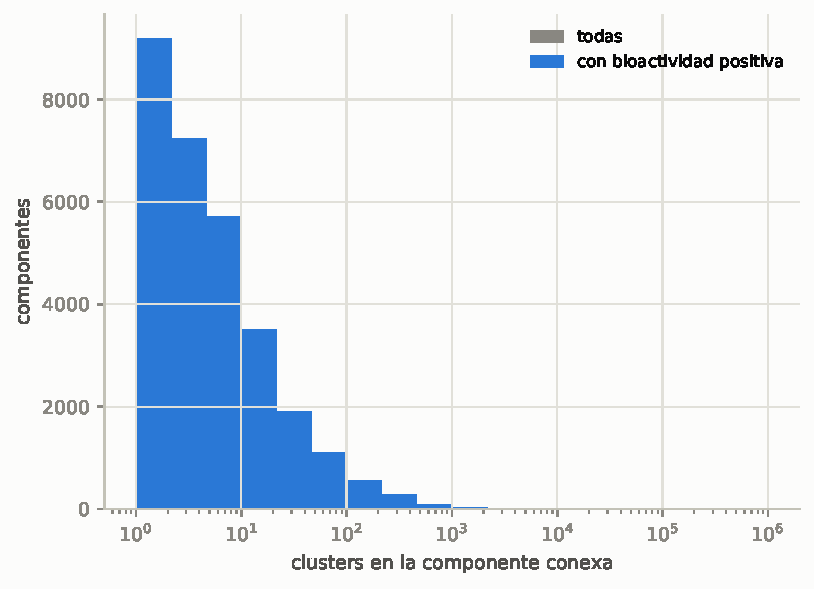
\includegraphics[width=.72\textwidth]{figuras/02_f02_componentes_conexas.pdf}
\caption{Tamaño de las componentes conexas del grafo de similitud química. Las
dos series se superponen: tras el recorte no queda ninguna componente sin
bioactividad positiva. Es una verificación de que el recorte hizo exactamente lo
que declara.}
\label{fig:comp}
\end{figure}

La desigualdad de evidencia entre organismos, que es la premisa del método,
abarca más de un orden de magnitud: entre \DrugMin\ y \DrugMax\ proteínas con
actividad conocida según el organismo (Figura~\ref{fig:disp}). Los organismos se
identifican por código y por tipo; el nombre no se publica en ninguna parte del
repositorio.

\begin{figure}[h]
\centering
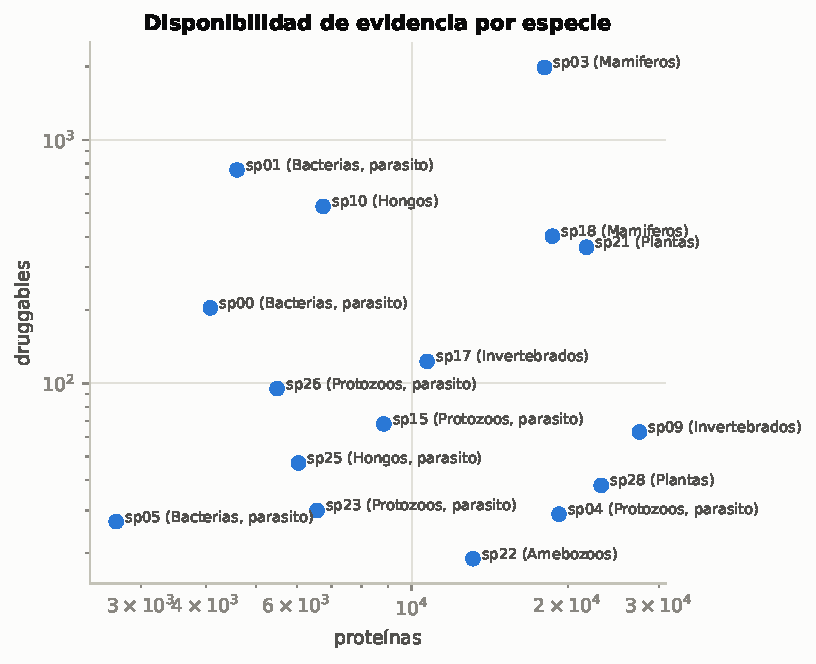
\includegraphics[width=.72\textwidth]{figuras/01_f01_disponibilidad.pdf}
\caption{Evidencia disponible por organismo, en escala logarítmica en los dos
ejes.}
\label{fig:disp}
\end{figure}

\section{El método}

Las anotaciones se puntúan primero por cuánto se enriquecen en proteínas ya
conocidas como blanco: un test exacto de Fisher unilateral por categoría,
corregido por comparaciones múltiples con Benjamini--Hochberg
\cite{benjamini1995}. Esa puntuación pondera después la propagación hacia las
proteínas sin evidencia. El esquema completo, con sus cuatro parámetros, es el
de \cite{berenstein2016}.

La métrica es el área parcial bajo la curva ROC restringida a
\(\mathrm{FPR}\le 0.10\), corregida por McClish \cite{mcclish1989} para que el
azar valga \(0.5\) y el clasificador perfecto \(1.0\). La restricción no es
cosmética: sólo importa el extremo del ranking, porque nadie va a ensayar
experimentalmente más allá de las primeras decenas de proteínas.

Un detalle de implementación con consecuencia numérica: la pAUC se calcula
interpolando el punto exacto \((\mathrm{FPR}_{\max}, \mathrm{TPR})\) antes de
integrar. Truncar en el último punto con \(\mathrm{FPR}\le \mathrm{FPR}_{\max}\),
que es lo directo, subestima el área.

La validación es \emph{leave-one-species-out}: para evaluar un organismo se
retira toda su evidencia de la semilla y se lo prioriza como si no se supiera
nada de él. Que eso esté bien hecho no se asume, se verifica: hay una prueba
dedicada que comprueba que ninguna proteína del organismo evaluado sobrevive en
la semilla, con su control negativo al lado.

\section{Resultados}

En su óptimo, la priorización alcanza una mediana de \AUCMediana\ de AUC01 entre
los \NEspeciesOpt\ organismos evaluados, con un rango de \AUCMin\ a \AUCMax, y
supera el azar en \NSobreAzar\ de ellos (Figura~\ref{fig:auc}).

\begin{figure}[h]
\centering
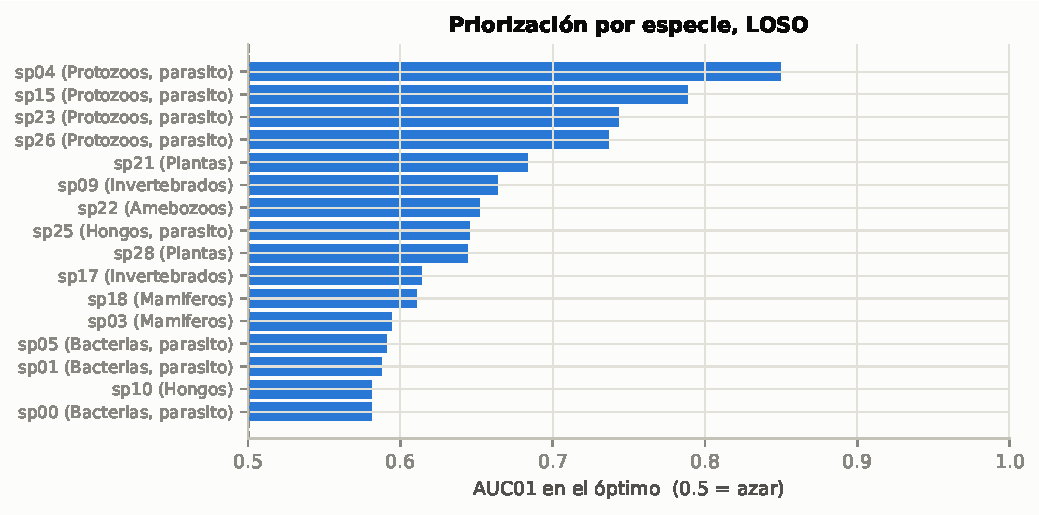
\includegraphics[width=.72\textwidth]{figuras/01_f03_auc01_por_especie.pdf}
\caption{Desempeño por organismo en su óptimo, bajo leave-one-species-out. La
línea punteada marca el azar.}
\label{fig:auc}
\end{figure}

Un número óptimo sólo significa algo si el óptimo no es un pico casual. La
Figura~\ref{fig:plateau} muestra cuán plano es: el desempeño se sostiene en un
entorno amplio de la grilla de parámetros, de modo que la elección no es frágil.

\begin{figure}[h]
\centering
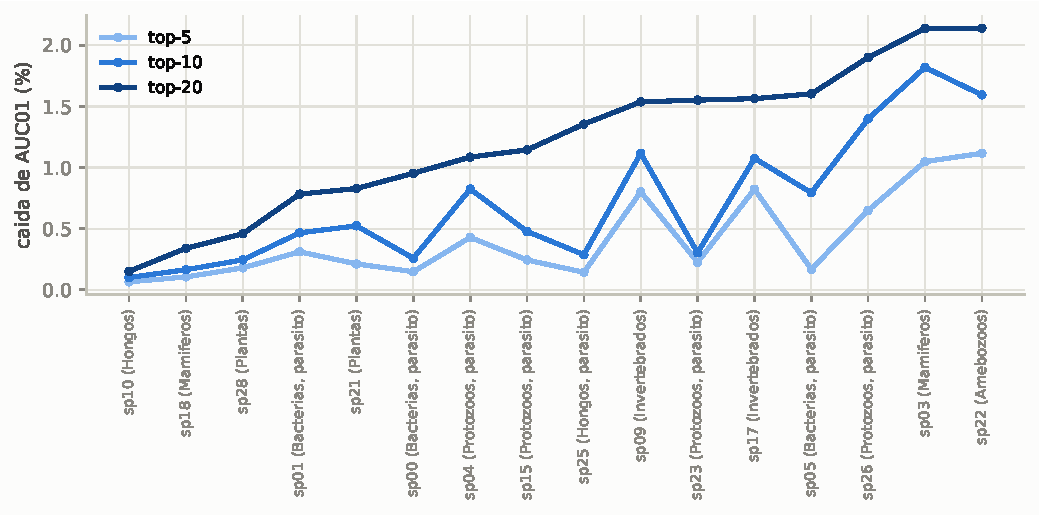
\includegraphics[width=.72\textwidth]{figuras/02_f03_plateau.pdf}
\caption{Estabilidad del óptimo en la grilla de parámetros.}
\label{fig:plateau}
\end{figure}

\section{Verificación}

Tres controles, del más barato al más caro.

\textbf{Las pruebas.} \NPruebas\ pruebas que corren en unos quince segundos:
integridad de las tablas, ausencia de fuga en la validación cruzada, las
métricas contra valores de referencia, las rutas y el entorno.

\textbf{El control externo.} Los óptimos por organismo se contrastan contra los
de una corrida independiente anterior, versionada en el repositorio. Los
parámetros óptimos coinciden en los \NEspeciesOpt\ organismos y la diferencia
máxima de AUC01 es \emph{exactamente} cero: la reproducción sobre la base
codificada no movió un solo dígito del control.

\textbf{El oráculo.} Las mismas tablas calculadas antes del recorte y de la
codificación. La comparación es informativa por una asimetría: el recorte
\emph{debe} mover los descriptivos de la base, y \emph{no debe} mover la
priorización, que no la toca. De \NComparadas\ columnas comparadas,
\NIdenticas\ resultan idénticas, \NExplicadas\ cambian de forma explicada por
el recorte y \NDiscrepancias\ quedan como discrepancia.

El corte cae donde tiene que caer: en \texttt{genome\_prioritization} las 149
columnas comparadas son idénticas y ninguna cambia, mientras que en
\texttt{huerfanas}, que construye la semilla desde el vecindario químico, 83 de
177 se mueven. La diferencia se explica sin apelar a nada externo: el conjunto
evaluado es el mismo --- 7\,782 pseudohuérfanas de los dos lados --- pero el filtro
de promiscuidad pasó de descartar 30 compuestos a \NPromiscuos, porque 23 de
aquellos 30 no sobrevivieron al recorte, y con menos aristas descartadas más
drogas consiguen semilla.

Una corrección que conviene dejar escrita: al diseñar esta comparación agrupé
\texttt{huerfanas} con \texttt{genome\_prioritization} entre lo que «no debería
moverse». Era incorrecto, y la corrida lo mostró. El criterio correcto es uno
solo: si el análisis toca la capa química, el recorte lo mueve.

\subsection*{Lo que casi sale mal}

Cuatro errores merecen quedar escritos, porque ninguno se encontró leyendo el
código: los encontraron las pruebas o la inspección de las salidas.

La base codificada guarda el tag de actividad como el entero \(2\), mientras el
código heredado filtraba por el texto \texttt{"positive"}. Esa comparación no
lanza ningún error: devuelve cero filas. El análisis completo seguía adelante
produciendo \texttt{NaN} y rankings vacíos, con \NPositivos\ enlaces de evidencia
descartados en silencio.

El segundo: InterPro y OrthoMCL se codificaron por separado, cada uno empezando
en cero, de modo que sus códigos se pisan --- los \NInterPro\ dominios caen
dentro del rango de los \NOrthoMCL\ grupos de ortología. Concatenarlos habría
fusionado anotaciones sin relación alguna, y el test de Fisher habría contado
proteínas de dos vocabularios distintos como si fueran de uno.

El tercero y el cuarto son el mismo patrón otra vez, y aparecieron ya con los
notebooks corriendo. Un filtro escrito como \texttt{sp\_id != "bioactive"}
compara un entero contra un texto y por lo tanto es siempre verdadero: la
pseudo-especie que agrupa blancos sin organismo asignado nunca se excluía, y
aportaba 67\,587 falsas pseudohuérfanas sobre un total de 127\,840 --- el 53\,\%
del conjunto. Y las relaciones de subestructura leídas de los datos crudos
entraban sin recodificar, de modo que no cruzaban contra la base y el filtro de
promiscuidad descartaba 30 compuestos falsos en lugar de \NPromiscuos\
verdaderos.

Los cuatro comparten la misma forma: una columna que pasó a ser un entero
codificado, comparada contra el texto que solía contener. Ninguno lanza una
excepción; todos devuelven un conjunto vacío o equivocado y dejan que el
análisis siga. Es la razón de que las pruebas vayan antes que los resultados, y
de que los números se lean de las tablas en vez de escribirse a mano.

\section{Procedencia y límites}

Cada corrida deja un \texttt{meta.json} junto a sus tablas con la fecha, el
notebook de origen, los parámetros, la fecha de cada tabla de entrada y las
versiones de python (\VersionPython) y pandas (\VersionPandas). El registro
completo de decisiones, con lo que se descartó en cada bifurcación y qué es
código propio frente a qué se llamó de una librería, está en
\texttt{PROVENANCE.md}.

Este repositorio no reproduce tres cosas, y conviene decirlo: la base misma, que
se deriva de datos que no se publican; los nombres legibles de las anotaciones,
que exigen un diccionario privado; y la identidad de los organismos, que es
deliberada. Lo que sí se publica es la salida de cada uno de esos pasos y el
registro de cómo se produjo.

\bibliographystyle{plain}
\bibliography{refs}

\end{document}
